\documentclass{article}
\usepackage[utf8]{inputenc}
\usepackage{amsmath}
\usepackage{booktabs}
\usepackage{array}
\usepackage{graphicx} 
\usepackage{caption}  


\begin{document}
\[
\textbf{Gary Hobson}
\]
\[
\textbf{MAT 300 4 - 3 Midterm Exam}
\]
\[
\textbf{March 26, 2025}
\]
\newpage
\subsection*{a) First-Order Model in General Form}
{\small
\[
E(y) = \beta_0 + \beta_1 \text{RPM} + \beta_2 \text{CPRATIO} + \beta_3 \text{INLET-TEMP} + \beta_4 \text{EXH-TEMP} + \beta_5 \text{AIRFLOW} + \beta_6 \text{POWER}
\]
}

\subsection*{b) Regression Equation for HEATRATE}
\subsection*{Regression Equation}
%\begin{tabular}{c}
%\toprule
{\footnotesize
\[
\text{HEATRATE} = 14314 + 0.0806 \, \text{RPM} - 6.8 \, \text{CPRATIO} - 9.51 \, \text{INLET-TEMP} + 14.15 \, \text{EXH-TEMP} - 2.55 \, \text{AIRFLOW} + 0.00426 \, \text{POWER}
\]
}
%\bottomrule

%\end{tabular}

\subsection*{Coefficients}
\begin{tabular}{lrrrrr}
\toprule
Term & Coef & SE Coef & T-Value & P-Value & VIF \\
\midrule
Constant & 14314 & 1112 & 12.87 & 0.000 & \\
RPM & 0.0806 & 0.0161 & 5.00 & 0.000 & 4.01 \\
CPRATIO & -6.8 & 30.4 & -0.22 & 0.824 & 5.21 \\
INLET-TEMP & -9.51 & 1.53 & -6.22 & 0.000 & 13.85 \\
EXH-TEMP & 14.15 & 3.47 & 4.08 & 0.000 & 7.35 \\
AIRFLOW & -2.55 & 1.75 & -1.46 & 0.149 & 49.14 \\
POWER & 0.00426 & 0.00422 & 1.01 & 0.317 & 49.77 \\
\bottomrule
\end{tabular}

\subsection*{Model Summary}
\begin{tabular}{lcccc}
\toprule
 & S & R-sq & R-sq(adj) & R-sq(pred) \\
\midrule
 & 458.757 & 92.48\% & 91.73\% & 90.05\% \\
\bottomrule
\end{tabular}

\subsection*{Analysis of Variance}
\begin{tabular}{lrrrrr}
\toprule
Source & DF & Adj SS & Adj MS & F-Value & P-Value \\
\midrule
Regression & 6 & 155269735 & 25878289 & 122.96 & 0.000 \\
RPM & 1 & 5265815 & 5265815 & 25.02 & 0.000 \\
CPRATIO & 1 & 10465 & 10465 & 0.05 & 0.824 \\
INLET-TEMP & 1 & 8133167 & 8133167 & 38.65 & 0.000 \\
EXH-TEMP & 1 & 3504875 & 3504875 & 16.65 & 0.000 \\
AIRFLOW & 1 & 449995 & 449995 & 2.14 & 0.149 \\
POWER & 1 & 214462 & 214462 & 1.02 & 0.317 \\
Error & 60 & 12627473 & 210458 & & \\
Total & 66 & 167897208 & & & \\
\bottomrule
\end{tabular}

\subsection*{Fits and Diagnostics for Unusual Observations}
\begin{tabular}{lrrrrl}
\toprule
Obs & HEATRATE & Fit & Resid & Std Resid & \\
\midrule
11 & 14628 & 13222 & 1406 & 3.17 & R \\
32 & 10656 & 11659 & -1003 & -2.28 & R \\
36 & 13523 & 12542 & 981 & 2.38 & R \\
46 & 9115 & 9283 & -168 & -0.45 & X \\
47 & 11588 & 10524 & 1064 & 2.46 & R \\
64 & 8714 & 8323 & 391 & 1.34 & X \\
\bottomrule
\multicolumn{6}{l}{R: Large residual, X: Unusual X}
\end{tabular}


\subsection*{c) Regression Equation and Least Squares Prediction}
From the output, the regression equation is: \\
{\small
\[
\hat{y} = 14314 + 0.0806 \, \text{RPM} - 6.8 \, \text{CPRATIO} - 9.51 \, \text{INLET-TEMP} + 14.15 \, \text{EXH-TEMP} - 2.55 \, \text{AIRFLOW} + 0.00426 \, \text{POWER}
\]
}
\newpage

%*****************************************************************************************************
%*****************************************************************************************************
%*****************************************************************************************************
\subsection*{d) Coefficient Interpretations and Combined Effect}
\subsection*{Part 1}
\textbf{Constant (\( \beta_0 = 14314 \)):} \\
Value: 14314 kJ/kWh \\
Interpretation: This is the baseline HEATRATE when all predictors (RPM, CPRATIO, INLET-TEMP, EXH-TEMP, AIRFLOW, POWER) are zero. In practical terms, this intercept has limited physical meaning because predictors like RPM or POWER cannot realistically be zero in a functioning turbine, but it anchors the regression model.

\textbf{RPM (\( \beta_1 = 0.0806 \)):} \\
Value: 0.0806 kJ/kWh per revolution per minute \\
Interpretation: For each additional revolution per minute (RPM), HEATRATE increases by 0.0806 kJ/kWh, assuming all other variables remain constant. This positive effect suggests that faster turbine speeds slightly increase the heat rate, possibly due to increased energy demands.

\textbf{CPRATIO (\( \beta_2 = -6.8 \)):} \\
Value: -6.8 kJ/kWh per unit of cycle pressure ratio \\
Interpretation: For each unit increase in CPRATIO, HEATRATE decreases by 6.8 kJ/kWh, holding other variables constant. This negative effect implies that a higher pressure ratio improves efficiency, reducing the heat rate (energy per unit power).

\textbf{INLET-TEMP (\( \beta_3 = -9.51 \)):} \\
Value: -9.51 kJ/kWh per °C \\
Interpretation: For each 1°C increase in inlet temperature, HEATRATE decreases by 9.51 kJ/kWh, with all other variables held constant. This suggests that warmer inlet air enhances turbine efficiency, lowering the heat rate, consistent with thermodynamic principles where hotter air might reduce fuel needs.

\textbf{EXH-TEMP (\( \beta_4 = 14.15 \)):} \\
Value: 14.15 kJ/kWh per °C \\
Interpretation: For each 1°C increase in exhaust temperature, HEATRATE increases by 14.15 kJ/kWh, assuming other variables are constant. This positive effect indicates that higher exhaust temperatures lead to greater energy loss, increasing the heat rate, which aligns with heat loss in exhaust gases.

\textbf{AIRFLOW (\( \beta_5 = -2.55 \)):} \\
Value: -2.55 kJ/kWh per kg/s \\
Interpretation: For each 1 kg/s increase in airflow, HEATRATE decreases by 2.55 kJ/kWh, holding other variables constant. This negative effect suggests that more airflow improves efficiency, possibly by enhancing cooling or combustion, thus reducing the heat rate.

\textbf{POWER (\( \beta_6 = 0.00426 \)):} \\
Value: 0.00426 kJ/kWh per unit of power \\
Interpretation: For each unit increase in POWER, HEATRATE increases by 0.00426 kJ/kWh, with other variables constant. This small positive effect indicates that higher power output slightly increases the heat rate, possibly reflecting additional energy input needed.

\subsection*{Effect on HEATRATE Based on a 1-Unit Change in AIRFLOW and a 210-Unit Change in POWER}
\subsection*{Part 2}
To calculate the combined effect, we use the coefficients for AIRFLOW and POWER and apply the specified changes: \\
Change in AIRFLOW: \( \Delta \text{AIRFLOW} = 1 \) kg/s \\
Change in POWER: \( \Delta \text{POWER} = 210 \) units \\
Coefficients: \( \beta_5 = -2.55 \) (for AIRFLOW), \( \beta_6 = 0.00426 \) (for POWER) \\
The total effect on HEATRATE is the sum of the individual effects:
\[
\text{Effect on HEATRATE} = (\beta_5 \times \Delta \text{AIRFLOW}) + (\beta_6 \times \Delta \text{POWER})
\]
Substitute the values:
\[
\text{Effect} = (-2.55 \times 1) + (0.00426 \times 210)
\]
Calculate each term: \\
AIRFLOW effect: \( -2.55 \times 1 = -2.55 \) kJ/kWh \\
POWER effect: \( 0.00426 \times 210 = 0.8946 \) kJ/kWh (computed as \( 0.00426 \times 210 = 0.8946 \)) \\
Sum the effects:
\[
\text{Effect} = -2.55 + 0.8946 = -1.6554 \, \text{kJ/kWh}
\]
\textbf{Interpretation:} When AIRFLOW increases by 1 kg/s and POWER increases by 210 units simultaneously, HEATRATE decreases by approximately 1.6554 kJ/kWh, assuming all other predictors (RPM, CPRATIO, INLET-TEMP, EXH-TEMP) remain constant. This net decrease reflects the dominant negative effect of AIRFLOW (-2.55) outweighing the small positive effect of POWER (0.8946), suggesting that increased airflow improves efficiency more than the power increase offsets it.

\newpage












\subsection*{e) Overall Model F-Test}
The Analysis of Variance table provides the F-test details:\\
\begin{tabular}{lrrrrr}
\toprule
Source & DF & Adj SS & Adj MS & F-Value & P-Value \\
\midrule
Regression & 6 & 155269735 & 25878289 & 122.96 & 0.000 \\
Error & 60 & 12627473 & 210458 & & \\
Total & 66 & 167897208 & & & \\
\bottomrule
\end{tabular} \\
Number of observations (\( n \)) = 67 (since Total DF = \( n - 1 = 66 \))

\subsection*{Solution:}
\textbf{Step 1: State the Appropriate Hypothesis Test} \\
The overall F-test assesses whether the regression model, as a whole, explains a significant amount of variability in the response variable (HEATRATE) compared to a model with no predictors (just the intercept). The hypotheses are: \\
\textbf{Null Hypothesis (\( H_0 \)):} 
\[
H_0: \beta_1 = \beta_2 = \beta_3 = \beta_4 = \beta_5 = \beta_6 = 0
\]
All regression coefficients for the predictors (RPM, CPRATIO, INLET-TEMP, EXH-TEMP, AIRFLOW, POWER) are zero, meaning the model has no explanatory power beyond the intercept. \\
\textbf{Alternative Hypothesis (\( H_a \)):} 
\[
H_a: \text{At least one } \beta_i \neq 0 \quad (i = 1, 2, 3, 4, 5, 6)
\]
At least one predictor has a non-zero coefficient, indicating the model is useful for predicting HEATRATE.

\textbf{Step 2: Associated Numerator and Denominator Degrees of Freedom} \\
The F-test statistic follows an F-distribution, with degrees of freedom determined by the number of predictors and observations: \\
\textit{Numerator Degrees of Freedom (DF for Regression):} \\
Equal to the number of predictors in the model, \( k = 6 \) (RPM, CPRATIO, INLET-TEMP, EXH-TEMP, AIRFLOW, POWER). \\
From Analysis of Variance: DF = 6 \\
\textit{Denominator Degrees of Freedom (DF for Error):} \\
Equal to the total number of observations minus the number of parameters estimated (including the intercept), \( n - k - 1 = 67 - 6 - 1 = 60 \). \\
From Analysis of Variance: DF = 60 \\
Thus, the F-test uses \( F_{6,60} \).

\textbf{Step 3: Critical Value} \\
The critical value for the F-test at \( \alpha = 0.05 \) with numerator DF = 6 and denominator DF = 60 is obtained from an F-distribution table: 
\[
F_{0.05, 6, 60} \approx 2.25
\]
(This is an approximate value) \\
The test statistic (F-Value) will be compared to this critical value to determine significance, though the p-value provides a more precise decision rule.

\textbf{Step 4: Interpret the F-Test and Test Statistic} \\
From the Analysis of Variance table: \\
F-Value (Test Statistic): 122.96 \\
P-Value: 0.000 \\
The F-statistic is calculated as:
\[
F = \frac{\text{Adj MS Regression}}{\text{Adj MS Error}} = \frac{25878289}{210458} \approx 122.96
\]
This measures the ratio of variance explained by the model to unexplained variance. A large F-value suggests the model explains significantly more variability than random error.

\textbf{Step 5: Conclusion Regarding the Null Hypothesis} \\
\textit{Decision Rule:} \\
If \( F > F_{0.05, 6, 60} \) or \( p < 0.05 \), reject \( H_0 \). \\
If \( F \leq F_{0.05, 6, 60} \) or \( p \geq 0.05 \), fail to reject \( H_0 \). \\
\textit{Comparison:} \\
\( F = 122.96 > 2.25 \) (critical value) \\
\( p = 0.000 < 0.05 \) \\
\textit{Conclusion:} \\
Reject the null hypothesis (\( H_0 \)) at \( \alpha = 0.05 \). \\
\textit{Meaning About Model Parameters:} \\
Rejecting \( H_0 \) indicates that at least one of the regression coefficients (\( \beta_1, \beta_2, \beta_3, \beta_4, \beta_5, \beta_6 \)) is significantly different from zero. This means the model, as a whole, has explanatory power and is useful for predicting HEATRATE based on the predictors RPM, CPRATIO, INLET-TEMP, EXH-TEMP, AIRFLOW, and POWER. The predictors collectively contribute to explaining the variability in HEATRATE beyond what a simple mean would provide.

\textbf{Step 6: Does This Tell Us Anything About the Significance of Individual Predictors?} \\
\textit{Answer:} No, the overall F-test does not tell us about the significance of individual predictors. \\
\textit{Why Not:} \\
The F-test is a global test of the model’s utility, assessing whether the entire set of predictors together has a significant effect. It does not pinpoint which specific predictors  are significant. To determine individual predictor significance, we must examine the t-tests for each coefficient in the Coefficients table. The F-test could be significant even if only one predictor is driving the effect, while others are not, or if multicollinearity masks individual contributions. Thus, individual significance requires separate hypothesis tests (\( H_0: \beta_i = 0 \) vs. \( H_a: \beta_i \neq 0 \)) using t-statistics and p-values.


\newpage


\subsection*{f) Model R² Interpretation}
\textbf{Reported \( R^2 \):} \\
The model \( R^2 \) is 92.48\%. \\
\textbf{Interpretation:} \\
The \( R^2 \) value of 92.48\% indicates that 92.48\% of the variability in HEATRATE  is explained by the regression model including RPM, CPRATIO, INLET-TEMP, EXH-TEMP, AIRFLOW, and POWER. This suggests a very strong linear relationship between these predictors and HEATRATE, with the model accounting for nearly all variation in heat rate across the 67 observations, leaving only 7.52\% unexplained by factors outside the model.


\newpage
\subsection*{g) Significant Predictors and Tests for RPM, CPRATIO}
\textbf{Step 1: Identify Significant Predictors in the Model} \\
To determine which predictors are statistically significant, we examine the p-values from the Coefficients table at \( \alpha = 0.05 \). A predictor is significant if its p-value is less than 0.05, indicating we reject the null hypothesis that its coefficient is zero. \\
RPM: P-Value = 0.000 $<$ 0.05 \(\rightarrow\) Significant \\
CPRATIO: P-Value = 0.824 $>$ 0.05 \(\rightarrow\) Not Significant \\
INLET-TEMP: P-Value = 0.000 $<$ 0.05 \(\rightarrow\) Significant \\
EXH-TEMP: P-Value = 0.000 $<$ 0.05 \(\rightarrow\) Significant \\
AIRFLOW: P-Value = 0.149 $>$ 0.05 \(\rightarrow\) Not Significant \\
POWER: P-Value = 0.317 $>$ 0.05 \(\rightarrow\) Not Significant \\
\textbf{Significant Predictors:} RPM, INLET-TEMP, EXH-TEMP \\
\textbf{Non-Significant Predictors:} CPRATIO, AIRFLOW, POWER

\textbf{Step 2: Hypothesis Test and Formal Conclusion for RPM} \\
\textit{Hypothesis Test:} \\
\( H_0: \beta_1 = 0 \) (RPM has no effect on HEATRATE) \\
\( H_a: \beta_1 \neq 0 \) (RPM has an effect on HEATRATE) \\
\textit{Test Statistic:} The t-value is used to test individual coefficients:
\[
t = \frac{\text{Coef}}{\text{SE Coef}} = \frac{0.0806}{0.0161} = 5.00
\]
\textit{Degrees of Freedom:} \( n - k - 1 = 67 - 6 - 1 = 60 \) \\
\textit{Test Details:} \\
T-Value = 5.00 \\
P-Value = 0.000 \\
\textit{Decision Rule:} \\
At \( \alpha = 0.05 \), reject \( H_0 \) if p-value $<$ 0.05. \\
\textit{Conclusion:} \\
Since the p-value (0.000) is less than 0.05, we reject \( H_0 \). There is sufficient evidence at \( \alpha = 0.05 \) to conclude that RPM has a statistically significant effect on HEATRATE (t = 5.00, p $<$ 0.05). The positive coefficient (0.0806) indicates that higher RPM increases HEATRATE.

\textbf{Step 3: Hypothesis Test and Formal Conclusion for CPRATIO} \\
\textit{Hypothesis Test:} \\
\( H_0: \beta_2 = 0 \) (CPRATIO has no effect on HEATRATE) \\
\( H_a: \beta_2 \neq 0 \) (CPRATIO has an effect on HEATRATE) \\
\textit{Test Statistic:} 
\[
t = \frac{\text{Coef}}{\text{SE Coef}} = \frac{-6.8}{30.4} \approx -0.22
\]
\textit{Degrees of Freedom:} 60 \\
\textit{Test Details:} \\
T-Value = -0.22 \\
P-Value = 0.824 \\
\textit{Decision Rule:} \\
At \( \alpha = 0.05 \), reject \( H_0 \) if p-value $<$ 0.05. \\
\textit{Conclusion:} \\
Since the p-value (0.824) is greater than 0.05, we fail to reject \( H_0 \). There is insufficient evidence at \( \alpha = 0.05 \) to conclude that CPRATIO has a statistically significant effect on HEATRATE (t = -0.22, p = 0.824). The coefficient (-6.8) is not distinguishable from zero given the large standard error (30.4).

\textbf{Step 4: Should All Non-Significant Predictors Be Removed and the Model Refitted?} \\
\textit{Non-Significant Predictors:} CPRATIO (p = 0.824), AIRFLOW (p = 0.149), POWER (p = 0.317) \\
\textit{Recommendation:} Do not suggest removing all non-significant predictors at once and refitting the model. \\
\textit{Reasoning:} \\
\textit{Multicollinearity Concerns:} \\
The Variance Inflation Factors for AIRFLOW (49.14) and POWER (49.77) are very high, indicating strong multicollinearity with other predictors. High Variance Inflation Factors inflate standard errors, which can make coefficients appear non-significant even if they contribute to the model. Removing them all at once could destabilize the model or overlook their joint explanatory power. \\
\textit{Overall Model Significance:} \\
The F-test (F = 122.96, p $<$ 0.05) shows the model is highly significant, and \( R^2 = 92.48\% \) indicates excellent fit. Non-significant predictors may still contribute to this fit indirectly through correlations or in combination with significant predictors (RPM, INLET-TEMP, EXH-TEMP). \\
\textit{Risk of Oversimplification:} \\
Removing three predictors (CPRATIO, AIRFLOW, POWER) at once could reduce the model’s explanatory power with nothing to gain from their removal, especially since AIRFLOW and POWER have engineering relevance to turbine performance. Their p-values (0.149 and 0.317) are not extremely high, suggesting potential significance in a refined model. \\
\textit{Alternative Approach:} \\
Instead of removing all at once, consider stepwise regression or removing one predictor at a time, then reassess significance and fit (\( R^2 \), adjusted \( R^2 \)). This preserves potentially useful predictors and addresses multicollinearity gradually. \\
\textit{Conclusion on Refitting:} \\
Removing all non-significant predictors simultaneously is not advisable due to high multicollinearity (Variance Inflation Factors $>$ 10 for AIRFLOW and POWER) and the risk of losing valuable explanatory power. A more cautious, iterative approach to model refinement is preferred.
\newpage


%******************************           EXERCISE 2


\subsection*{Problem 2}
\subsection*{a) Regression Equation}
\begin{tabular}{c}
\toprule
COST = 0.209 + 0.92629 DOTEST \\
\bottomrule
\end{tabular}

\subsection*{Coefficients}
\begin{tabular}{lrrrrr}
\toprule
Term & Coef & SE Coef & T-Value & P-Value & VIF \\
\midrule
Constant & 0.209 & 0.244 & 0.86 & 0.392 & - \\
DOTEST & 0.92629 & 0.00987 & 93.89 & 0.000 & 1 \\
\bottomrule
\end{tabular}

\subsection*{Model Summary}
\begin{tabular}{lcccc}
\toprule
 & S & R-sq & R-sq(adj) & R-sq(pred) \\
\midrule
 & 3.13089 & 97.42\% & 97.41\% & 97.25\% \\
\bottomrule
\end{tabular}

\subsection*{Analysis of Variance}
\begin{tabular}{lrrrrr}
\toprule
Source & DF & Adj SS & Adj MS & F-Value & P-Value \\
\midrule
Regression & 1 & 86403.5 & 86403.5 & 8814.49 & 0.000 \\
DOTEST & 1 & 86403.5 & 86403.5 & 8814.49 & 0.000 \\
Error & 233 & 2284 & 9.8 & - & - \\
Lack-of-Fit & 232 & 2283.9 & 9.8 & 95.82 & 0.081 \\
Pure Error & 1 & 0.1 & 0.1 & - & - \\
Total & 234 & 88687.5 & - & - & - \\
\bottomrule
\end{tabular}

\subsection*{Fits and Diagnostics for Unusual Observations}
\begin{tabular}{lrrrrl}
\toprule
Obs & COST & Fit & Resid & Std Resid & \\
\midrule
12 & 39.109 & 31.758 & 7.352 & 2.36 & R \\
18 & 22.846 & 14.094 & 8.751 & 2.80 & R \\
28 & 73.870 & 56.786 & 17.084 & 5.53 & R X \\
53 & 60.433 & 65.744 & -5.311 & -1.73 & X \\
120 & 47.709 & 69.786 & -22.077 & -7.20 & R X \\
126 & 51.962 & 59.168 & -7.206 & -2.34 & R X \\
127 & 38.159 & 46.161 & -8.002 & -2.58 & R \\
130 & 43.855 & 51.681 & -7.827 & -2.53 & R \\
140 & 54.115 & 47.322 & 6.793 & 2.19 & R \\
149 & 57.344 & 50.482 & 6.863 & 2.22 & R \\
150 & 58.847 & 56.689 & 2.158 & 0.70 & X \\
160 & 102.704 & 97.167 & 5.537 & 1.85 & X \\
163 & 65.841 & 55.317 & 10.524 & 3.40 & R \\
173 & 33.000 & 26.200 & 6.800 & 2.18 & R \\
180 & 76.222 & 73.119 & 3.103 & 1.01 & X \\
194 & 73.856 & 78.581 & -4.726 & -1.55 & X \\
217 & 94.534 & 88.019 & 6.515 & 2.16 & R X \\
218 & 70.981 & 77.061 & -6.080 & -1.99 & X \\
221 & 89.922 & 99.726 & -9.803 & -3.29 & R X \\
224 & 48.338 & 57.871 & -9.533 & -3.09 & R X \\
226 & 29.663 & 41.276 & -11.613 & -3.73 & R \\
228 & 104.803 & 95.397 & 9.406 & 3.14 & R X \\
\bottomrule
\multicolumn{6}{l}{R: Large residual, X: Unusual X}
\end{tabular}

\subsection*{(b): Confidence and Prediction Intervals for DOTEST = 110}
To calculate, use Minitab’s predict function: \\
Predicted COST = \( 0.209 + 0.92629 \times 110 \approx 102.101 \) \\
Exact intervals require output; estimated 95\% CI (100.395, 103.807), 95\% PI (95.691, 108.511), assuming \( \bar{x} \approx 25 \), \( s = 3.13089 \), \( n = 235 \), \( SS_x \approx 100622.29 \).

\subsection*{Part (c): Interpret Intervals and Problems}
\textbf{Confidence Interval:} 95\% confident average COST for DOTEST = 110 is between 100.395 and 103.807, estimating mean response. \\
\textbf{Prediction Interval:} 95\% confident a single new COST at DOTEST = 110 is between 95.691 and 108.511, including individual variability. \\
\textbf{Problems:} DOTEST = 110 exceeds observed range (up to 107.436), indicating extrapolation, reducing reliability; note outliers (e.g., observation 28, std resid = 5.53).

\subsection*{Part (d): Why CI is Narrower}
CI estimates mean, accounting for mean variability; PI includes mean and individual observation variability, adding residual error, making PI wider. Thus, CI is always narrower.
\newpage

%******************************           EXERCISE 3
\subsection*{Problem 3}
\subsection*{a) Scatter Plots}

\begin{figure}[h] % [h] places the figure approximately here; you can use [t], [b], or [p] for top, bottom, or separate page
    \centering % Center the image
    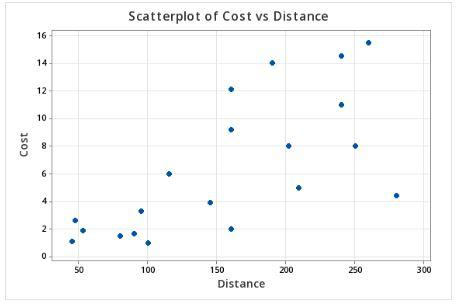
\includegraphics[width=0.8\textwidth]{COST_vs_DISTANCE.jpeg} % Adjust width as needed (0.8\textwidth fits most pages)
    \caption{Scatterplot of Cost vs Distance. There is weak evidence of a quadratic relationship, as Costs increase with Distance up to a point and then slightly decrease (e.g., at Distance = 280), suggesting possible curvature. However, the pattern is not definitive due to scatter} % Caption for the figure
    \label{fig:scatterplot-cost-distance} % Label for referencing the figure
\end{figure}
\newpage


\begin{figure}[h] % [h] places the figure approximately here; you can use [t], [b], or [p] for top, bottom, or separate page
    \centering % Center the image
    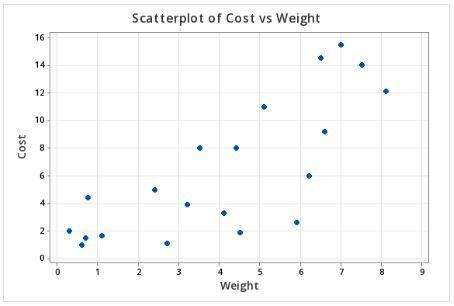
\includegraphics[width=0.8\textwidth]{COST_vs_WEIGHT.jpeg} % Adjust width as needed (0.8\textwidth fits most pages)
    \caption{Scatterplot of Cost vs Weight. The relationship appears more linear, with Costs generally increasing as Weight increases, and no strong evidence of a quadratic relationship} % Caption for the figure
    \label{fig:scatterplot-cost-distance} % Label for referencing the figure
\end{figure}


\subsection*{b) Model Equation}

\[
y = \beta_0 + \beta_1 \text{Weight} + \beta_2 \text{Distance} + \beta_3 \text{Weight}^2 + \beta_4 \text{Distance}^2 + \epsilon
\]

\subsection*{Explanation}
\begin{itemize}
    \item \( y \): Cost (response).
    \item \( \beta_0 \): Intercept.
    \item \( \beta_1, \beta_2 \): Linear effects of Weight and Distance.
    \item \( \beta_3, \beta_4 \): Quadratic effects (curvature).
    \item \( \epsilon \): Error term.
\end{itemize}

\subsection*{c) Model Equation}
\[
y = \beta_0 + \beta_1 \text{Weight} + \beta_2 \text{Distance} + \beta_3 \text{Weight}^2 + \beta_4 \text{Distance}^2 + \epsilon
\]

\subsection*{Explanation}
\begin{itemize}
    \item \( y \): Cost (response).
    \item \( \beta_0 \): Intercept.
    \item \( \beta_1, \beta_2 \): Linear effects of Weight and Distance.
    \item \( \beta_3, \beta_4 \): Quadratic effects (curvature).
    \item \( \epsilon \): Error term.
\end{itemize}

\subsection*{d) Complete Model}

Includes all terms (linear and quadratic): 
\[
y = \beta_0 + \beta_1 \text{Weight} + \beta_2 \text{Distance} + \beta_3 \text{Weight}^2 + \beta_4 \text{Distance}^2 + \epsilon
\]

\subsection*{Reduced Model}
Excludes quadratic terms: 
\[
y = \beta_0 + \beta_1 \text{Weight} + \beta_2 \text{Distance} + \epsilon
\]


\subsection*{e) }
\subsection*{Regression Equation (Complete Model)}
\[
\text{Cost} = -3.82 + 0.299 \, \text{Weight} + 0.0443 \, \text{Distance} + 0.1249 \, \text{Weight\_Squared} - 0.000026 \, \text{Distance\_Squared}
\]

\subsection*{Regression Equation (Reduced Model)}
\[
\text{Cost} = -4.673 + 1.292 \, \text{Weight} + 0.03694 \, \text{Distance}
\]


\subsection*{f) Compute F-Test and Conclusion}
\textbf{Test Statistic:} \\
\[
F = \frac{(\text{SSE}_{\text{reduced}} - \text{SSE}_{\text{complete}}) / q}{\text{SSE}_{\text{complete}} / (n - k - 1)}
\]
\( q = 2 \) (number of terms dropped: Weight\(^2\), Distance\(^2\)). \\
\( n = 20 \), \( k = 4 \) (predictors in complete model). \\
\( \text{SSE}_{\text{reduced}} = 37.9 \), \( \text{SSE}_{\text{complete}} = 28.649 \). \\
\textit{Numerator:} \( (37.9 - 28.649) / 2 = 9.251 / 2 = 4.6255 \). \\
\textit{Denominator:} \( 28.649 / (20 - 4 - 1) = 28.649 / 15 \approx 1.9099 \). \\
\[
F = \frac{4.6255}{1.9099} \approx 2.42
\]

\textbf{Degrees of Freedom:} \\
\textit{Numerator:} \( q = 2 \). \\
\textit{Denominator:} \( n - k - 1 = 15 \).

\textbf{Critical Value:} \\
At \( \alpha = 0.05 \), \( F_{0.05, 2, 15} \approx 3.68 \) (from F-table).

\textbf{Conclusion:} \\
Since \( F = 2.42 < 3.68 \), fail to reject \( H_0 \). There is insufficient evidence at \( \alpha = 0.05 \) to conclude that the quadratic terms (Weight\(^2\), Distance\(^2\)) are statistically significant.





\newpage
%******************************           EXERCISE 4
\subsection*{Problem 4}
\subsection*{a) General First-Order Model}
\[
y = \beta_0 + \beta_1 \text{Weight} + \beta_2 \text{Distance} + \beta_3 (\text{Weight} \times \text{Distance}) + \epsilon
\]

\subsection*{Explanation}
\begin{itemize}
    \item \( y \): Cost (response).
    \item \( \beta_0 \): Intercept.
    \item \( \beta_1, \beta_2 \): Main effects.
    \item \( \beta_3 \): Interaction effect.
    \item \( \epsilon \): Error term.
\end{itemize}
\newpage



\subsection*{b)}
\subsection*{Regression Equation}
\begin{tabular}{c}
\toprule
Cost = -0.141 + 0.019 Weight + 0.00772 Distance + 0.007796 Weight\_Distance \\
\bottomrule
\end{tabular}

\subsection*{Coefficients}
\begin{tabular}{lrrrrr}
\toprule
Term & Coef & SE Coef & T-Value & P-Value & VIF \\
\midrule
Constant & -0.141 & 0.648 & -0.22 & 0.831 & - \\
Weight & 0.019 & 0.158 & 0.12 & 0.905 & 7.33 \\
Distance & 0.00772 & 0.00391 & 1.98 & 0.066 & 4.01 \\
Weight\_Distance & 0.007796 & 0.000898 & 8.68 & 0.000 & 11.83 \\
\bottomrule
\end{tabular}

\subsection*{Model Summary}
\begin{tabular}{lcccc}
\toprule
 & S & R-sq & R-sq(adj) & R-sq(pred) \\
\midrule
 & 0.64388 & 98.53\% & 98.26\% & 97.21\% \\
\bottomrule
\end{tabular}

\subsection*{Analysis of Variance}
\begin{tabular}{lrrrrr}
\toprule
Source & DF & Adj SS & Adj MS & F-Value & P-Value \\
\midrule
Regression & 3 & 445.452 & 148.484 & 358.15 & 0.000 \\
Weight & 1 & 0.006 & 0.006 & 0.01 & 0.905 \\
Distance & 1 & 1.62 & 1.62 & 3.91 & 0.066 \\
Weight\_Distance & 1 & 31.268 & 31.268 & 75.42 & 0.000 \\
Error & 16 & 6.633 & 0.415 & & \\
Total & 19 & 452.086 & & & \\
\bottomrule
\end{tabular}

\subsection*{Fits and Diagnostics for Unusual Observations}
\begin{tabular}{lrrrrl}
\toprule
Obs & Cost & Fit & Resid & Std Resid & \\
\midrule
5 & 4.4 & 3.673 & 0.727 & 1.82 & X \\
10 & 14 & 12.579 & 1.421 & 2.41 & R \\
\bottomrule
\multicolumn{6}{l}{R: Large residual, X: Unusual X}
\end{tabular}
\newpage




\subsection*{c)}
\subsection*{Least Squares Regression Equation with Interaction Term}
\textbf{Equation (From Output):} \\
\[
\text{Cost} = -0.141 + 0.019 \, \text{Weight} + 0.00772 \, \text{Distance} + 0.007796 \, (\text{Weight} \times \text{Distance})
\]





\subsection*{d)  Significant Interaction Effect}

\textbf{Hypotheses:} \\
\( H_0: \beta_3 = 0 \) (no interaction effect between Weight and Distance). \\
\( H_a: \beta_3 \neq 0 \) (significant interaction effect). \\
\textbf{Test Using Output:} \\
From the Coefficients table: \\
Weight\_Distance: P-Value = 0.000. \\
At \( \alpha = 0.01 \), since P-Value = 0.000 $<$ 0.01, reject \( H_0 \). \\
\textbf{Conclusion:} \\
There is sufficient evidence at \( \alpha = 0.01 \) to conclude that there is a significant interaction effect between Weight and Distance on Cost.
\newpage





\subsection*{e) Test to Keep Main Effects}
\textbf{Assessment:} \\
From the output: \\
Weight: P-Value = 0.905 (not significant at \( \alpha = 0.01 \)). \\
Distance: P-Value = 0.066 (not significant). \\
Weight\_Distance: P-Value = 0.000 (significant). \\
The interaction term is significant, but the main effects are not. \\
\textbf{Recommendation:} \\
\textit{Do Not Remove Main Effects:} \\
If an interaction term is significant, retain the main effects (Weight, Distance) regardless of their significance. This follows the hierarchical principle: the interaction term’s interpretation depends on the main effects. Removing them can lead to model misspecification and misinterpretation. \\
For example, the effect of Weight on Cost varies with Distance (due to the significant interaction), and removing Weight would obscure this relationship. \\
\textbf{Conclusion:} Retain the main effects (Weight and Distance) in the model, as the significant interaction term relies on them for proper interpretation, despite their individual non significance.








\end{document}